




\newpage

\section{Zeitlich veränderliches Magnetfeld}

\subsection{Induktion}

Bis jetzt haben wir elektrische und magnetische Grössen angeschaut, die sich zeitlich nicht ändern. \\
Sind beide Grössen konstant, so beeinflussen sie sich nicht. \\
Sobald sich jedoch der magnetische Fluss $\phi$  \textbf{zeitlich ändert}, besteht einen Zusammenhang zwischen Magnetfeld und elektrischem Feld. \\
Wie magnetischer Fluss und elektrisches Feld zusammenhängen beschreibt das \textbf{Induktionsgesetz}


\gl{Gleichung}{Induktionsgesetz}
\begingl
\formulaBegin
  $\displaystyle \oint_s \vec{E}\cdot d\vec{s} = -\frac{d}{dt}\Phi(t) =  -\frac{d}{dt} \big ( \iint_{A_s} \vec{B} \cdot d\vec{A} \big )$
\formulaEnd
\textbf{Variablen} \\
$B = $ Magnetische Flussdichte $[B] = T$\\
$A_s = $ Vom Weg S aufgespannte Fläche. $[A_s] = m^2$ \\

Falls B Feld konstant auf Fläche und senkrecht: \\

\formulaBegin
  $\displaystyle  \oint_s \vec{E}\cdot d\vec{s} = -\frac{d}{dt} \big ( B_{eff} \cdot A_s \big ) $
\formulaEnd
\iend


\newpage

Bewegen wir einen Leiter mit Lädungstrager in einem Magnetfeld, so wirkt eine magnetische Kraft auf die Ladungsträger im Leiter. \\
Die Ladungsträger werden sich desshalb in Richtung der Kraftwirkung bewegen. \\
Aufgrund dieser Bewegung, werden Ladungsträger \textbf{getrennnt}. Diese Trennung der Ladungsträger lösst ein elektrisches Feld aus, welches wir als Spannung messen können.

\begin{center}
  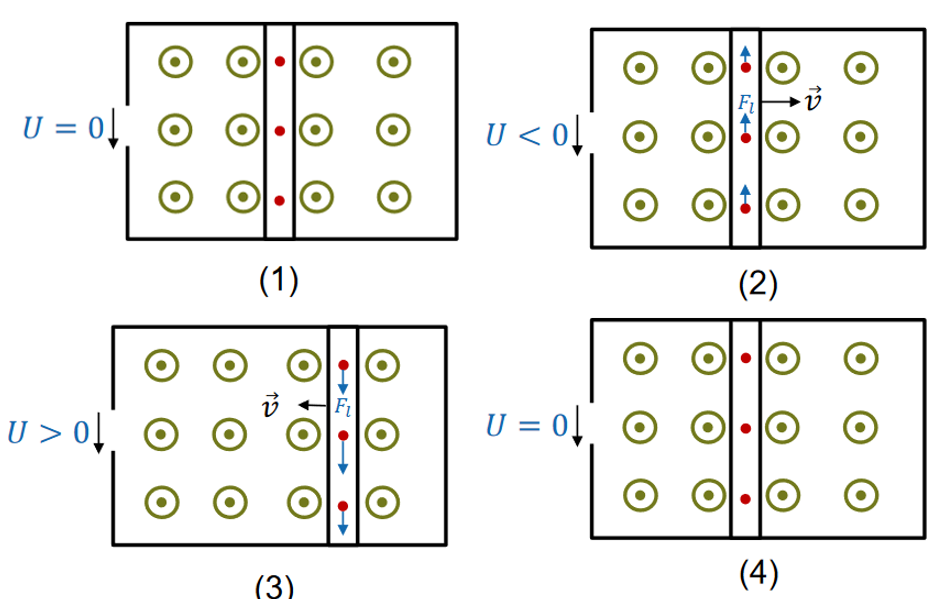
\includegraphics[scale=0.4]{img/beweg-ind} \\
  \textbf{Induzierte Spannung} \\
    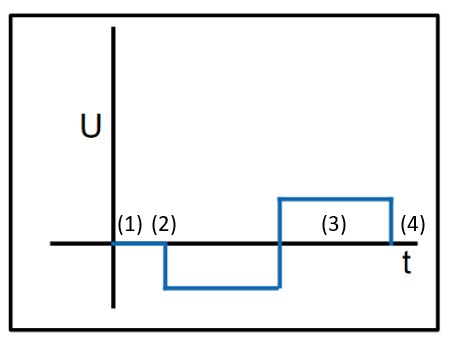
\includegraphics[scale=0.4]{img/beweg-ind-graph}
\end{center}



Die Lenzsche Regel gibt uns Informationen darüber, in welche Richtung sich Ladungsträger bei der Induktion bewegen werden.
\definition{Lenzsche Regel}
\beginip
\begin{center}
  \texttt{"}Der induzierte Strom ist stets so gerichtet, dass er der Ursache seiner Entstehung entgegenwirkt.  \texttt{"}
\end{center}
\iend
\newpage

\bsp{Beispiel}{Lemzsche Regel}
\beginbsp
Gegeben sei folgende Leiterschleife, welche sich nach Rechts in ein Magnetfeld bewegt. \\
Ziel dieser Aufgabe ist es, herauszufinden, in welche Richtung Spannung und Strom zeigen werden.
\begin{center}
  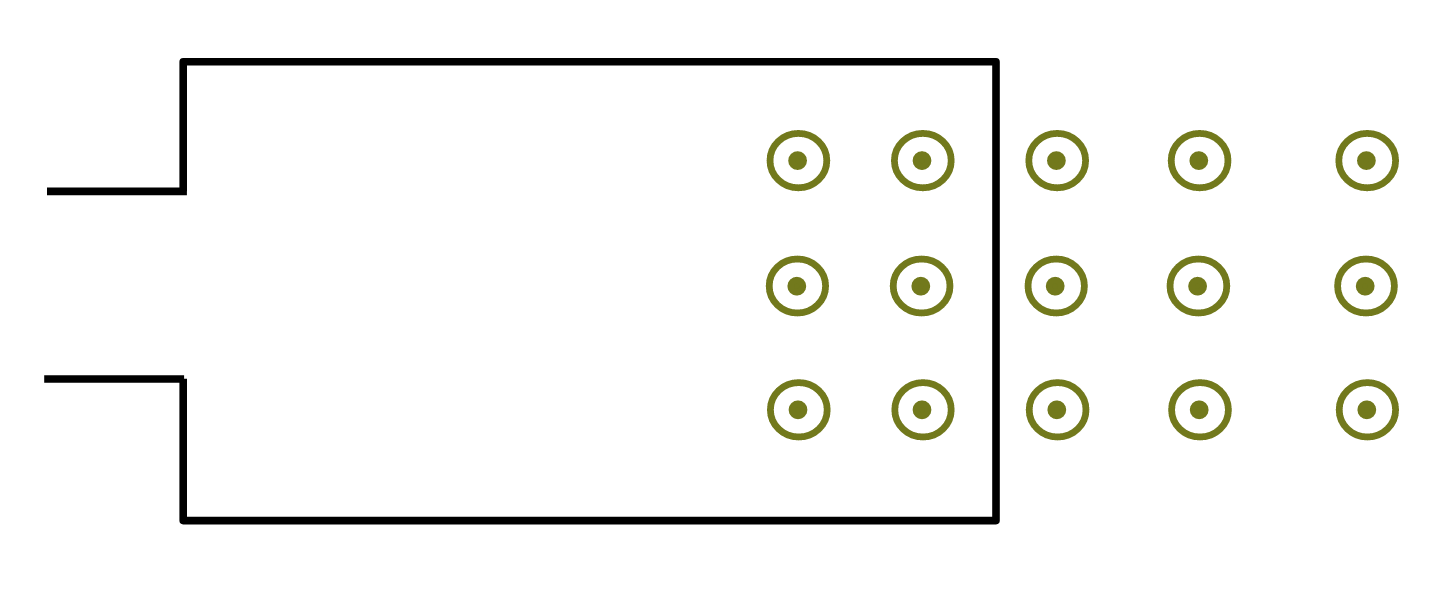
\includegraphics[scale=0.2]{img/ex-lenzsche-regel}
\end{center}

Bewegen wir unsere Leiterschleife nach Rechts weiter in unser Feld hinein, so schliessen wir \textbf{Magnetfeld} welche in unsere Richtung zeigt ein. \\
Das System selbst, möchte jedoch im Gleichgewicht bleiben, weswhalb es versucht ein Magnetfeld aufzubauen, welches der Änderung entgegenwirkt. (Siehe rotes Magnetfeld) \\
Um dieses Magnetfeld aufzubauen, ist ein Strom, der im Uhrzeigersinn fliesst, nötig. \\
Dieser Strom bringt positive Ladungsträger auf die untere Seite, weshalb eine Spannung in Richtung des eingezeichneten Pfeiles entsteht.


\begin{center}

  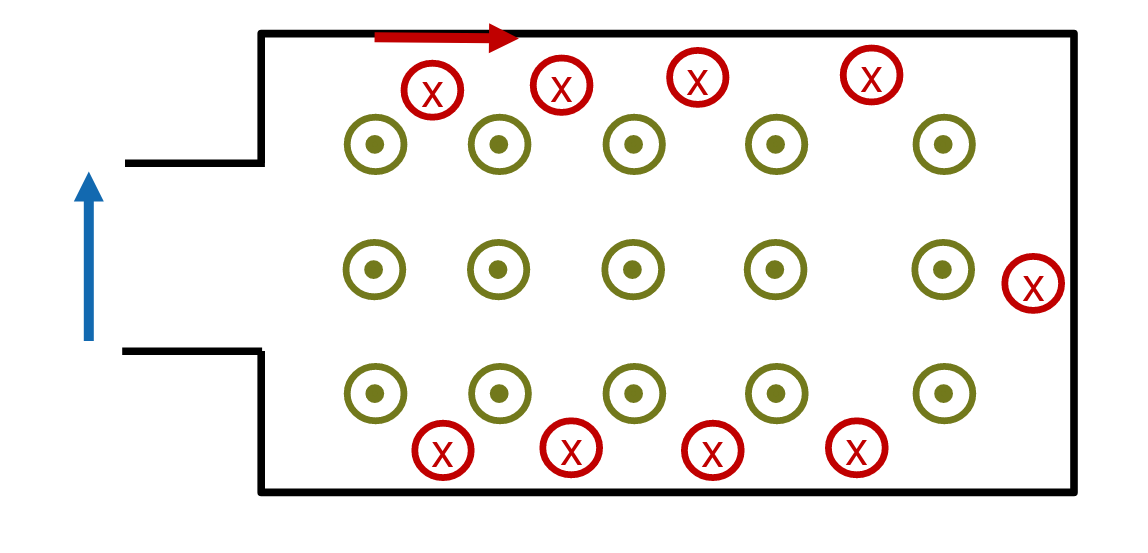
\includegraphics[scale=0.2]{img/ex-lenzsche-r-sol}
\end{center}
\iend

\newpage

\gl{Gleichung}{Bewegungsinduktion}
\begingl
Bewegen wir einen Leiter mit einer Geschwindigkeit in ein Magnetfeld , so wird ein elektrisches Feld induziert.

\formulaBegin
$ \displaystyle d\vec{E}_i = \vec{v} \times \vec{B}  \cdot dl$
\formulaEnd

\textbf{Variabeln}: \\
$ d\vec{E}_i =$ Induzierstes E-Feld auf dem kleinen Wegstück $dl$ \\
$ \vec{v} = $Geschwindigkeit des Leiterstückes $ dl $ \\
$ \vec{B} = $B-Feld \\

Um die induizierte Spannung zu berechnen, muss $d\vec{E}_i$ über die wirksame Leiterlänge im Magnetfeld $l$ integriert werden: \\
\formulaBegin
$\displaystyle U_{i} = \int_l  d\vec{E}_i = \int_l \vec{v} \times \vec{B}  \cdot d\vec{l} \underbrace{\simeq}_{B \perp V} B \cdot V \cdot l_{eff}$
\formulaEnd

\iend



\bsptask{Beispiel}{Bewegungsinduktion}
\beginbsp
  Wie gross ist die im Leiter induzierte Spannung u in Abhängigkeit der Zeit t, wenn der Leiter im Zeitpunkt t=0 entsprechend dem Bild in das Magnetfeld eintaucht?
\begin{center}
  \ibox{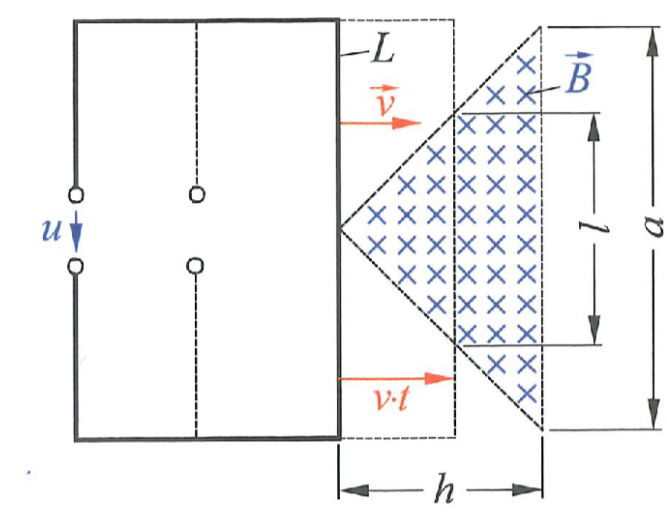
\includegraphics[scale=0.3]{img/a-bewegind}}
\end{center}
\iend
\newpage




\bsp{Lösung}{}
\beginbsp


\textbf{Lösung 1} Bewegungsinduktion \\
Mithilfe des Umlaufintegrales $\displaystyle \oint_s \vec{E} d\vec{s}$ erhalten wir folgenden Zusammenhang für das induzierte E-Feld und die gemessene Spannung:
\begin{center}
  $ \displaystyle u = \int_l \vec{E}_i \cdot d\vec{l} = \int_l \vec{v} \times \vec{B} \cdot d \vec{l}$
\end{center}
Da Geschwindigkeit und B-Feld immer senkrecht stehen, vereinfacht sich das Kreuzprodukt zu einer Multiplikation. \\
Da Leiterlänge und E-Feld parallel sind, vereinfacht sich das Integral zu einer Multiplikation
\begin{center}
  $\displaystyle u = B \cdot V \cdot l_{eff}$
\end{center}
Wobei $l_{eff}$ die \textbf{effektive Leiterlänge} $=$ die Leiterlänge im Magnetfeld beschreibt. \\
Diese Leiterlänge ist zeitlich abhängig. Aus dem Strahlensatz folgt
\begin{center}
  $\frac{l_{eff}(t)}{v \cdot t} = \frac{a}{h}$ \\
  $\rightarrow l_{eff} (t) =  \frac{a}{h} \cdot vt$
\end{center}
Somit gilt für die induzierte Spannung
\begin{center}

    $\displaystyle  \doubleunderline{ u} = B \cdot V \cdot l_{eff}(t) = B \cdot v \cdot  \frac{a}{h} \cdot vt =  \doubleunderline{ B \cdot v^2 \frac{a}{h} \cdot t}$
\end{center}

\textbf{Lösung 2} Induktionsgesetz \\
Wir verwenden das Induktionsgesetz
\begin{center}
  $\displaystyle \oint_s \vec{E} \cdot d\vec{s} = - \frac{d}{dt} \big( \phi (t)\big)$
\end{center}
Da Feld und Fläche senkrecht stehen gilt für den Fluss $\phi$
\begin{center}
  $\phi(t) = A_{eff}(t) \cdot B(t)$
\end{center}
Die Fläche welche vom Leiter umschlossen und vom Magnetfeld durchflossen wird berechnet sich zu
\begin{center}
  $A_{eff} (t) = \frac{1}{2} \big ( vt \cdot \frac{a}{h} \cdot vt \big) = \frac{1}{2} v^2t^2 \frac{a}{h}$
\end{center}
Somit gilt für den Fluss
\begin{center}
  $ \phi(t) =  B \cdot A_{eff}(t) = B \cdot \frac{1}{2} v^2t^2 \frac{a}{h}$
\end{center}
Und für das \textbf{rechtshändige Umlaufintegral} (Daumen zeigt in Richtung Fluss, Finger Richtung des geschlossenen Weges)
\begin{center}
  $ -u = - \frac{d}{dt} \big( \phi(t) \big) = - B v^2 t \frac{a}{h}$ \\
  $ \displaystyle \rightarrow \doubleunderline{ u = B v^2  \frac{a}{h} t }$
\end{center}
\iend

\newpage



Gemäss dem Induktionsgesetz, löst ein sich \textbf{zeitlich ändernder} Fluss eine Spannung aus. \\
Fliesst nun ein Strom durch eine Leiterschleife, so wird sich als Reaktion auf den Stromfluss ein magnetisches Feld innerhalb dieser Leiterschleife aufbauen.  \\
Verändert sich also der Strom, welcher die Schleife durchfliesst zeitlich, so ändert sich auch das magnetische Feld zeitlich, was zu einer Spannung an den Klemmen der Leiterschleife führt.

\gl{Gleichung}{Selbstinduktion}
\begingl
\begin{center}

\ibox{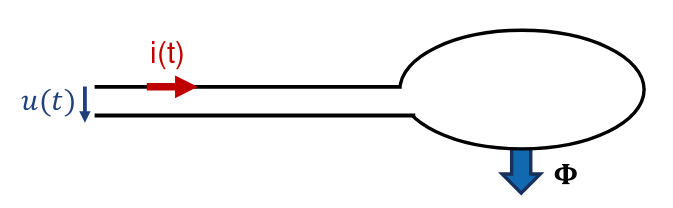
\includegraphics[scale=0.3]{img/selbstind}}
\fspace

\end{center}


\formulaBegin
$u(t) = L \cdot \frac{d}{dt}\big( i(t) \big) $
\formulaEnd
\textbf{Variabeln} \\
$L =$ Selbstinduktivität der Schleife $ [L] = H$ \\
$i(t) =$ Strom durch die Leiterschleife$ [i(t)] = A$ \\
$u(t) = $ Spannung an der Leiterschleife $[u(t)] = V$
\iend

\bsptask{Beispiel}{Selbstinduktion}
\beginbsp
Durch eine Spule mit Selbstinduktivität $L = 1 H$ fliesst der Strom $i(t)$ (Siehe Bild). \\
Zeichnen Sie graphisch die induzierte Spannung $u(t)$
\begin{center}
  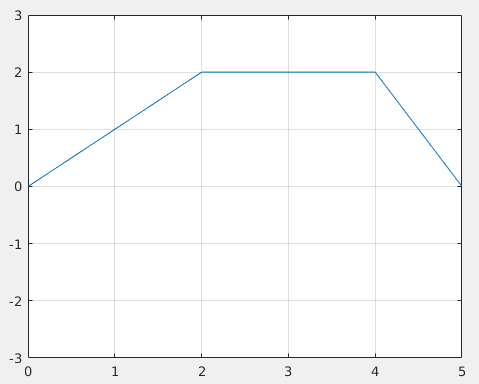
\includegraphics[scale=0.5]{img/selbstind-a1}
\end{center}

\iend


\newpage


\bsp{Lösung}{}
\beginbsp
Wir teilen den Strom in 3 Teilbereiche auf: \\
\textbf{1.} $t < 2$
\begin{center}

    $ i_1(t) = t \rightarrow u_1(t) = L \cdot \frac{d}{dt} t = 1V $
\end{center}
  \textbf{2.} $ 4 > t > 2$
  \begin{center}

      $ i_2(t) = 2A \rightarrow u_2(t) = L \cdot \frac{d}{dt} 2 A = 0V$
  \end{center}

    \textbf{3.} $t > 4$
    \begin{center}

        $ i_3(t) = -2 \cdot (t-4) + 2A \rightarrow u_3(t) = L \cdot \frac{d}{dt} \big( -2 \cdot (t-4) + 2A \big) = -2 V$
    \end{center}
\begin{center}
  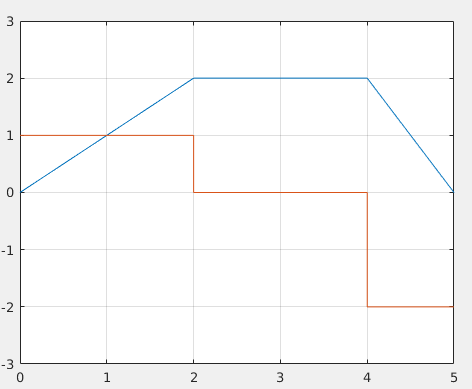
\includegraphics[scale=0.5]{img/selbstind-a1-lsg}
\end{center}
\iend



\newpage


\subsection{Charakteristische Gleichungen von Kapazität und Induktivität}
\gl{Gleichung}{Induktivität}
\begingl
Der Zusammenhang zwischen Strom und Spannung an der Induktivität ist wie folgt gegeben
\formulaBegin
$\displaystyle u_L(t) = L \cdot \frac{d}{dt}\big( i(t) \big)$

$\displaystyle  i_L(t) = i_l(0) + \frac{1}{L} \cdot \int_0^t u_L(\tau) d\tau$

\formulaEnd
%TODO IMAGE
\iend


\gl{Gleichung}{Kondensator}
\begingl
Der Zusammenhang zwischen Strom und Spannung am Kondensator ist wie folgt gegeben
\formulaBegin
$\displaystyle u_c(t) = u_c(0) + \frac{1}{C} \int_0^t i_c(\tau) d\tau$ \\

$\displaystyle i_c(t) = C \cdot \frac{d}{d t} \big(u_c(t) \big)$ \\
\formulaEnd
%TODO IMAGE
\iend


\textbf{Begründung} \\
Mit dem Wissen, dass Strom definiert ist als die Ladung pro Zeit $ \displaystyle \frac{dQ}{dt} = i$ folgt: \\
\begin{center}
	$\displaystyle \frac{\partial}{\partial t} (C \cdot u) = \frac{\partial}{\partial t} (Q) $ \\
	$ \displaystyle C \cdot \frac{du}{dt} = i \rightarrow u(t) = \frac{1}{C} \cdot \int_0^t i \cdot dt$
\end{center}
